\chapter{Biodiversity}
\section{Introduction to Biodiversity}

The 21st century marks the era of big data.
This increase of data has effected all spheres of science, especially the study of biodiversity''
Biodiversity data covers an increasingly wide range of areas including bio-geography, ecology, invasive species biology, and climate change.
The information collected in biodiversity informatics projects has been used for studies relating to food security, control of disease vectors, and marine productivity \cite{Barve}.  
\begin{figure}[htbp!] 
   \centering
   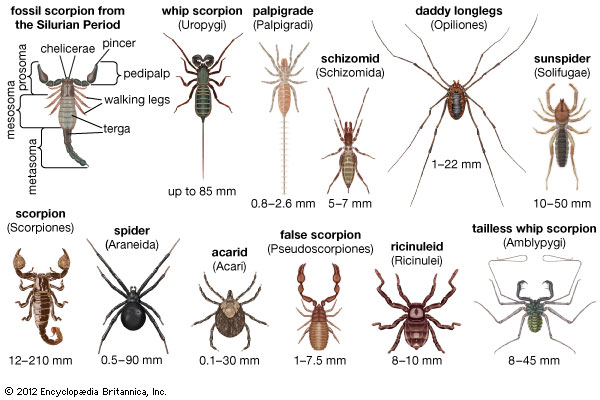
\includegraphics[width=0.5\textwidth]{pictures/biodiversity/spiders.jpg} 
   \caption{Example of biodiversity in arachnids}
   \label{fig:arachnids}
\end{figure}

Primary biodiversity data is one of the most important biodiversity statistics; it documents a species' occurrences in time and space.
Associated metadata, or data that describes statistics given in another set, may include information about who identified and recorded the species, who verified the identification, climatic parameters, micro-habitat information, number of individuals, sex, size, etc \cite{Barve}.
When these two types of data are formatted in universally accepted formats, published openly and integrated with other such data streams, they are known ``Digitally Accessible Knowledge'' or DAK.

There are many sources of biodiversity data including: directed surveys, broad-scale surveys, and biological collections. 

\subsection{Direct Surveys}

Directed surveys are often used where prior knowledge of a given system or biological mechanism exists.
Surveys for this type of experiment are designed to control for known sources of variation\cite {GBIFbirds}.
Direct surveys aim to establish a casual relationship between some experimental treatment and its effect and are widely accepted in the scientific community.
Regardless, the data collected in this type of survey is extremely expensive.
Additionally, the data is aggregated by many researchers working independently in small areas over small time scales, which creates a network of heterogeneous data repositories with little opportunity for integration and eventual data degradation.

\subsection{Broad  Surveys}

Broad-scale surveys involve over ten million observations annually.
This data is used to generate probabilistic estimates of species occurrence, which can then be used to determine general patterns over broad geographic regions and time scales \cite {GBIFbirds}.
Data for broad surveys can be collected by anyone, ranging from trained observers to interested citizens.
As a result, these surveys are relatively inexpensive to operate; however, the regulations behind these surveys are more relaxed, resulting in more potential for bias.
Nonetheless, these studies provide the bulk of non-specimen observational data available via the Internet \cite {SP}.

\subsection{Biological Collections}

Biological collections are data sets of specimens.
This type of data is primarily assembled to document the phenotypes and genotypes of the biotas worldwide \cite{Barve}.
Biological collections are typically considered as ``high-quality, low-volume'' sources of data on biological diversity \cite{Barve}.

Given all the different ways to collect data, each with their own pros and cons, it is important for researchers utilizing biodiversity data to determine the completeness and accuracy of their data sets.
Data visualization is one technique to observe patterns within very large data sets that are extremely difficult to analyze manually.
The goal of this study is to learn how analyze biodiversity data sets and visualize these sets in order to paint a comprehensive representation of the data.

\section{Objectives of the Case Study}

The bdvis packages allows users to create models that visualize the biodiversity of the data collected.
Using data that catalogs the occurrences of the species in question, bdvis creates a  heat-map with geography superimposed for every point on the globe where the species was recognized, create a temporal visualization of the data by day, week, or month, and create a chronohorogram which plots the number of records on each day with colors indicating the value, and concentric circles for each year.
The models that are created not only show the user if there is a lack of biodiversity, or lack of data, but also exactly where this lack occurs.
The user can also see variations in the data on different months, and days.
This variation in data may be due to differences in temperature.

By the end of this lesson, the reader should be able to:
\begin{enumerate}
\item Create a map of completeness of biodiversity
\item Visualize geographical and temporal coverage
\item Visualize gaps in data
\end{enumerate}

\section{Building the Model}

Before loading you data into RStudio, it is necessary to install the packages: \texttt{maps}, \texttt{sqldf}, \texttt{plotrix}, \texttt{treemap}, \texttt{plyr}, \texttt{ggplot2}, \texttt{grid}, \texttt{lattice}, \texttt{chron}, \texttt{devtools}, \texttt{bdvis}, and \texttt{rinat}.
After installing these packages, load them into your library.

\begin{lstlisting}
#make sure to include quotation marks when installing packages
install.packages("maps")
#leave off quotation marks when loading packages into library
library(maps)
\end{lstlisting}

Download the ``Historical bird ringing records'' from: \url{http://www.gbif.org/dataset/b4ae1720-1431-49ee-bfeb-8146fc42b1a3}.
After data is configured to fit the bdvis package, set the working directory to the location of the data on your laptop.
Next, read the data from the file, making sure to set \texttt{stringsAsFactors} as false.

\begin{lstlisting}
#set working directory to where data is located
setwd("/Users/margauxwinter/Desktop/Rfolder/dwca-safring-v1.0")

#read your data into RStudio
birds <- read.delim('occurrence.txt', quote='', stringsAsFactors=FALSE)
\end{lstlisting}

You may begin using functions that create visual models of the data.
The first model used in this example is a graph of completeness vs. number of species.
To create this graph use the function bdcomplete, which divides the extent of the dataset in cells, via the \texttt{getcellid} function.
Next, the function calculates the Chao2 estimator of species richness, which uses occurrence data from many samples to estimate the entirety of the species diversity.
This function requires a minimum number of records that must be present on each cell to properly compute the index.
If there are too few records in the cells, the function is unable to finish, an error will result.
Use the following code to generate the plot shown in figure \ref{fig:completeness}.

\begin{lstlisting}
comp=bdcomplete(birds)
\end{lstlisting}

\begin{figure}[htbp!]
   \centering
   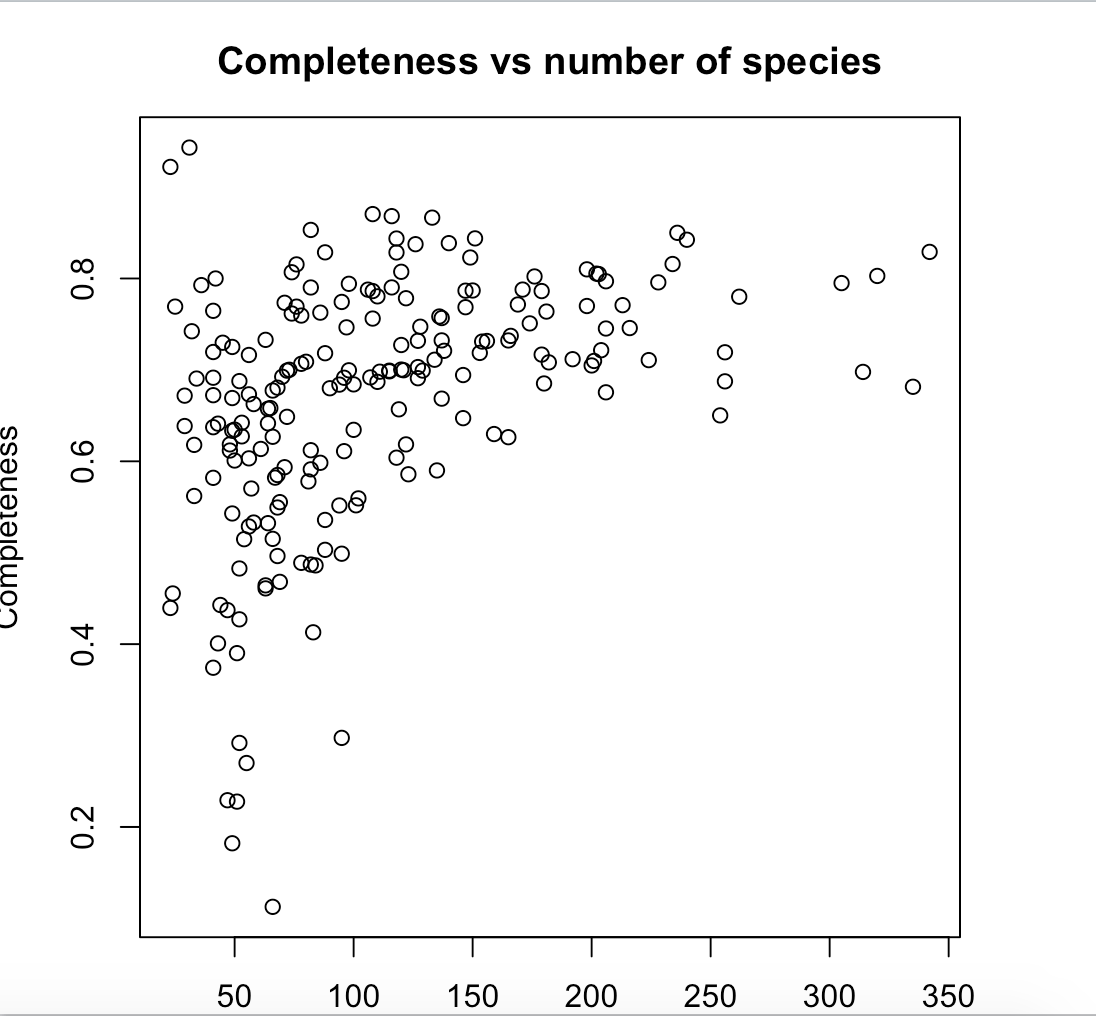
\includegraphics[width=0.5\textwidth]{pictures/biodiversity/complete.jpg} 
      \caption{Completeness}
   \label{fig:completeness}
\end{figure} 

Next use the function mapgrid, which builds a grid map colored according to the density of records in each cell.
Mapgrid allows the user to visually see gap and blank spaces in data.
Grids are 1-degree cells, build with the getcellid function.
Record-density maps apply a color gradient according to the number of records in the cell.
Species-density maps apply a color gradient according to the number of different species in the cell, disregarding the number of records.
Completeness maps apply a color gradient according to the completeness index, from 0 (incomplete) to 1 (complete).
Use the following function to generate a map grid as shown in figure \ref{fig:Mapgrid}

\begin{lstlisting}
mapgrid(comp,ptype='complete')
\end{lstlisting}

\begin{figure}[htbp!]
   \centering
   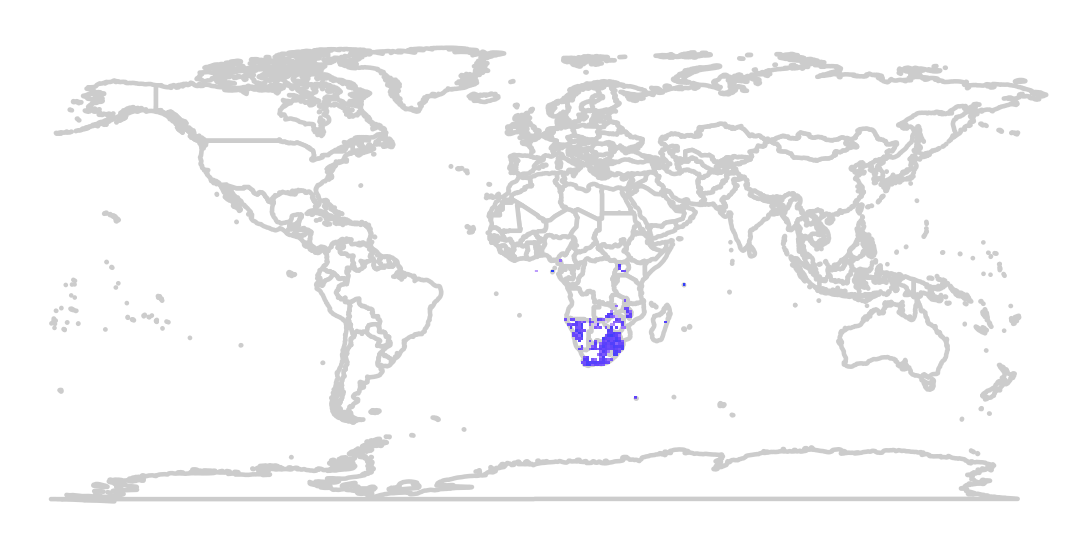
\includegraphics[width=0.5\textwidth]{pictures/biodiversity/map.jpg} 
      \caption{Mapgrid}
   \label{fig:Mapgrid}
\end{figure} 

In order to create a chronohorogram of the dates in the provided data set, use the function chronohorogram.
A chronohorogram plots the number of records on each day with colors indicating the value and concentric circles for each year.
The following code is used to create a chronohorogram like the one shown in figure \ref{fig:chronohorogram}.

\begin{lstlisting}
chronohorogram(birds)
\end{lstlisting}

\begin{figure}[htbp!] 
   \centering
      \caption{Chronohorogram}
   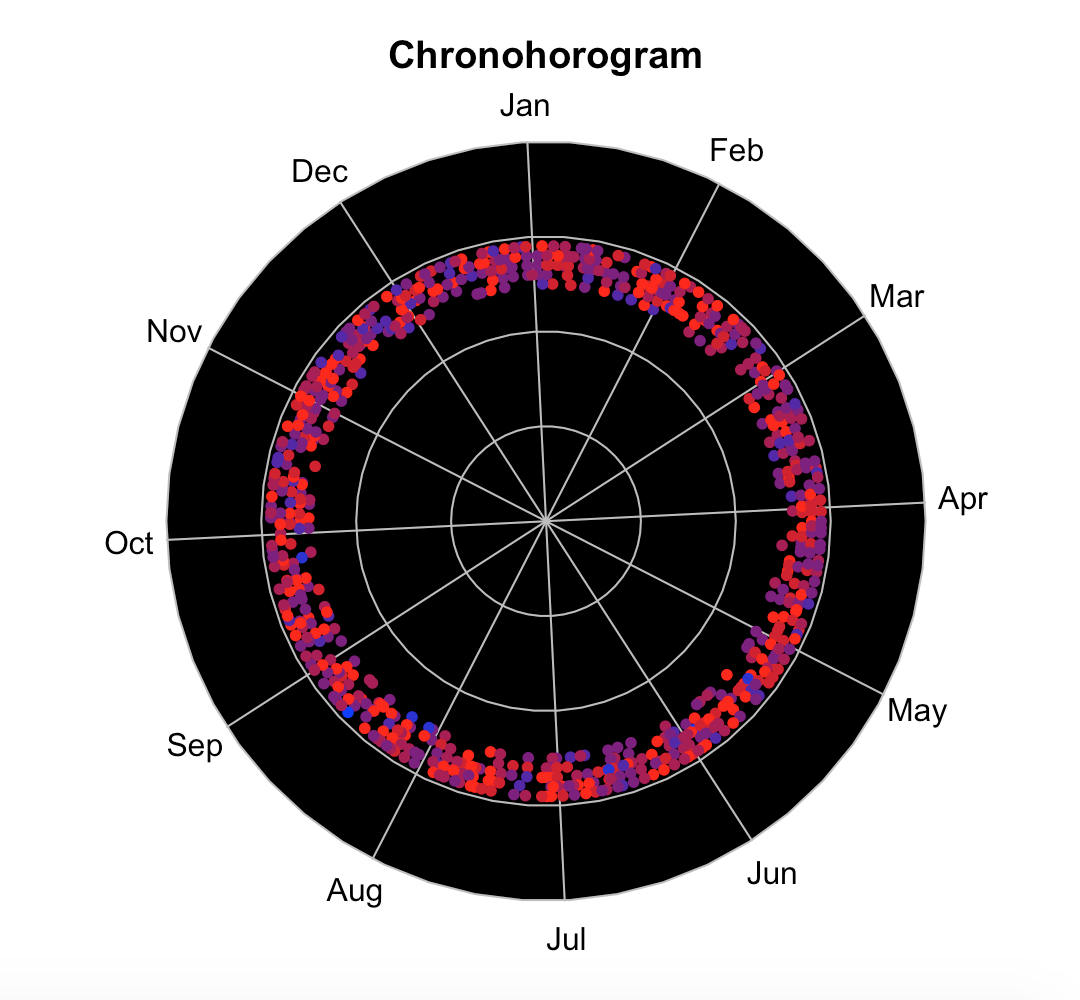
\includegraphics[width=0.5\textwidth]{pictures/biodiversity/chronohorogram.jpg} 
   \label{fig:chronohorogram}
\end{figure} 

Use the function \texttt{distrigraph} to build plots displaying distribution of biodiversity records among user-defined features.
The next four distrigraphs all use different p-types (feature to represent) allowing each graphic to depict different aspects of the data.
The following code is used to create all four distrigraphs respectively as shown in figures \ref{fig:distrigraph1} and \ref{fig:distrigraph2}.

\begin{lstlisting}
distrigraph(birds,ptype="cell",col="tomato")
distrigraph(birds,ptype="species",ylab="Species")
distrigraph(birds,ptype="efforts",col="red")
distrigraph(birds,ptype="efforts",col="red",type="s")
\end{lstlisting}
\begin{figure}[htbp!]
    \centering
   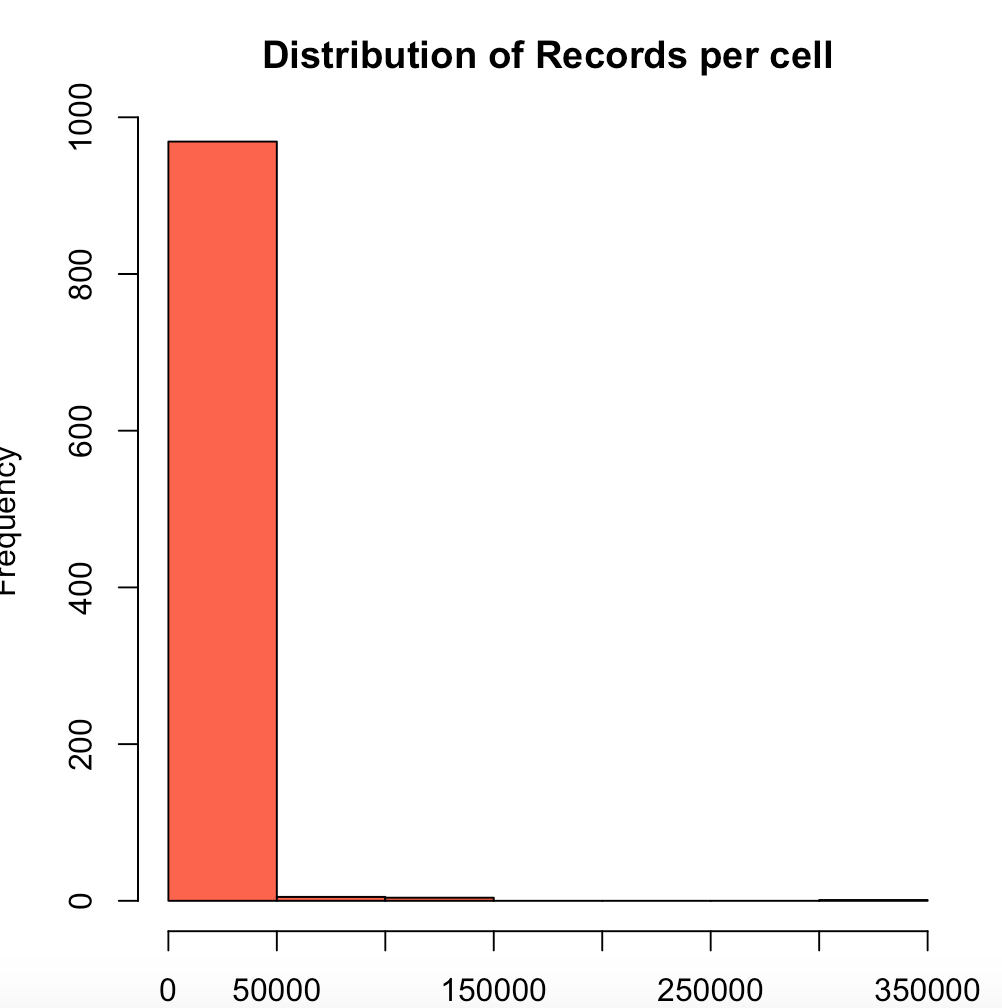
\includegraphics[scale=0.35]{pictures/biodiversity/distrograph1.jpg}
   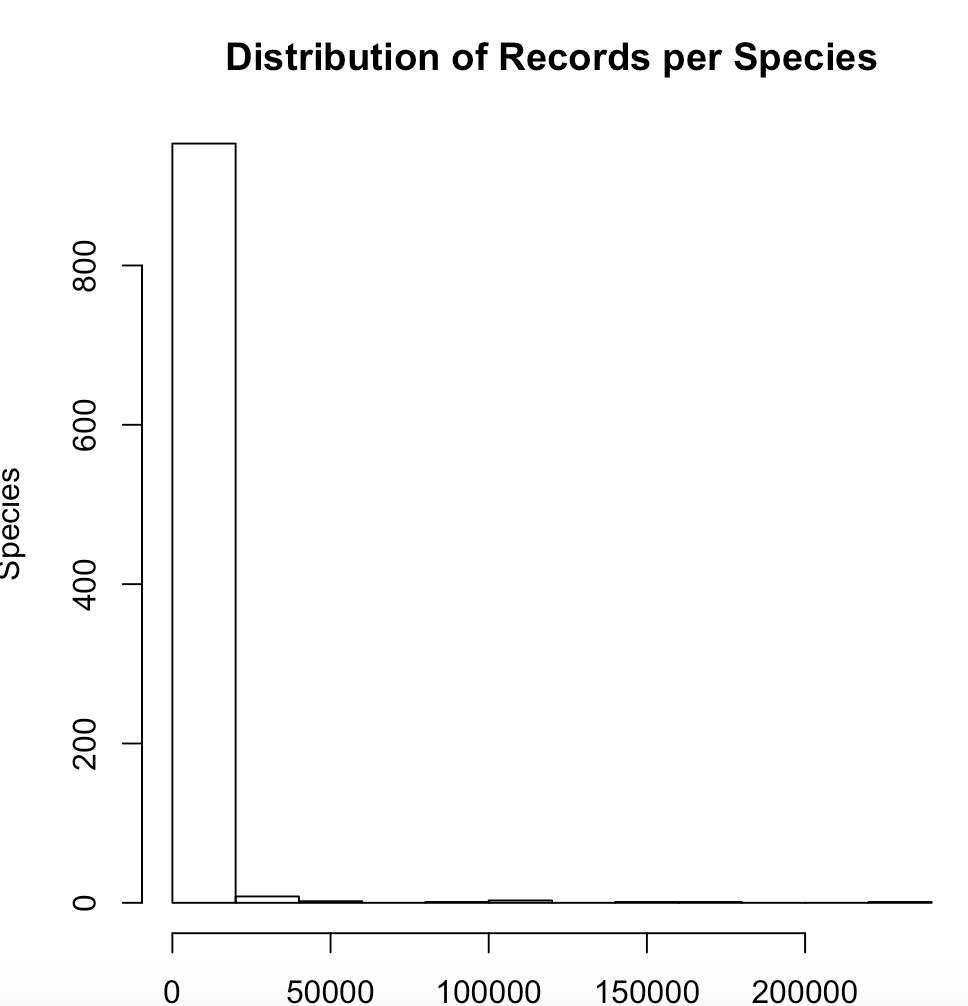
\includegraphics[scale=0.35]{pictures/biodiversity/distrograph2.jpg}
   \caption{Left: Distrigraph 1, Right: Distrigraph 2}
   \label{fig:distrigraph1}
\end{figure}


\begin{figure}[htbp!] 
   \centering
   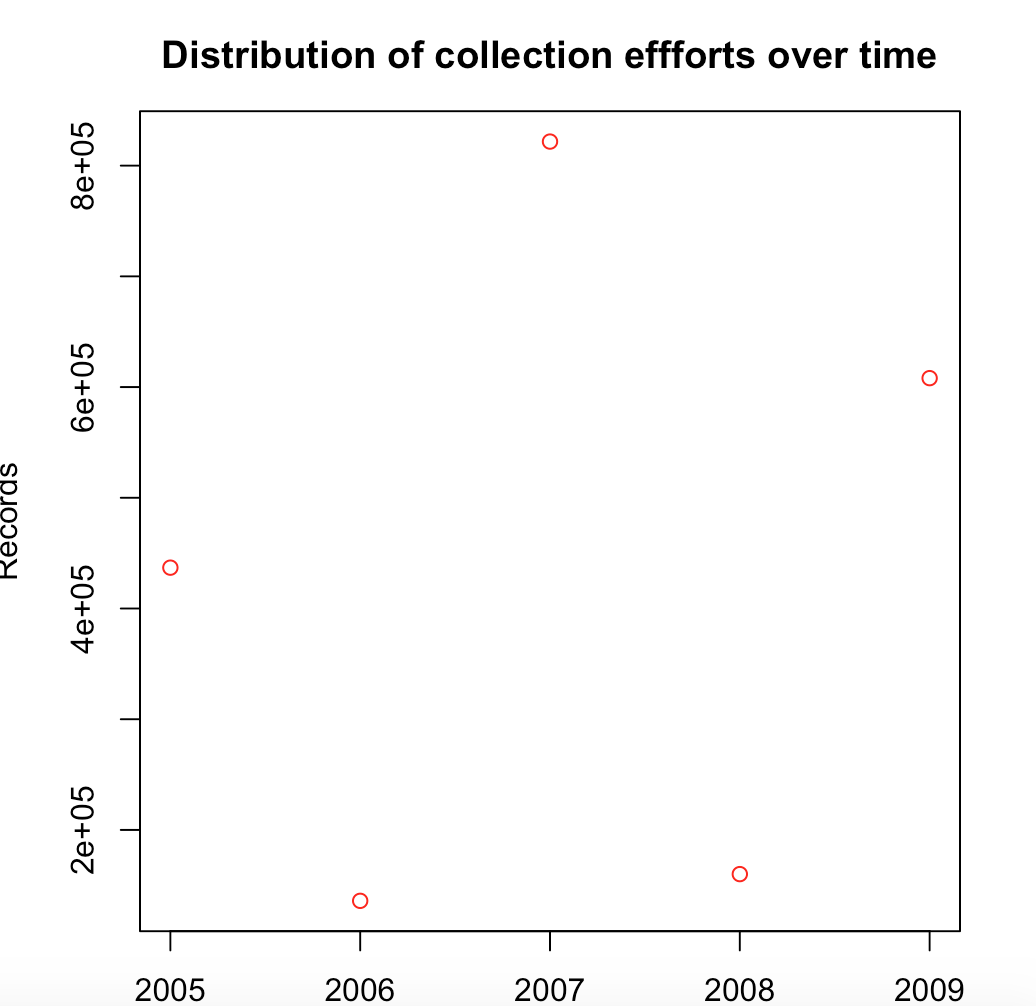
\includegraphics[scale=0.35]{pictures/biodiversity/distrograph3.jpg}
    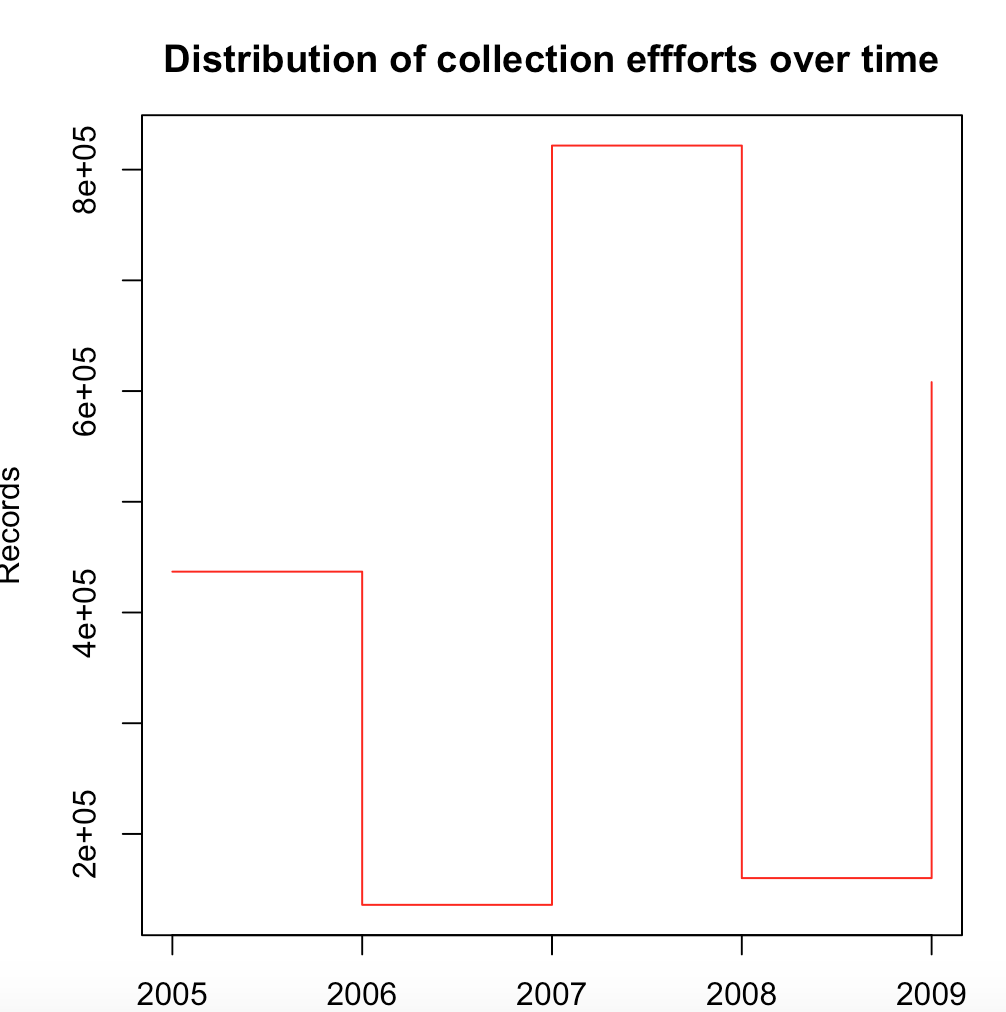
\includegraphics[scale=0.35]{pictures/biodiversity/distrograph4.jpg}
      \caption{Left: Distrigraph 3, Right: Distrigraph 4 }
    \label{fig:distrigraph2}
\end{figure}

Bdcalendarheat create a calendar heat map in which a calendar is structured as a matrix-like plot where each cell represents a unique date.
The cells are colored as to show the density of records for that date.
Use the following function to create the heat map shown in figure \ref{fig:heatcal}.

\begin{lstlisting}
bdcalendarheat(birds)
\end{lstlisting}

\begin{figure}[htbp!] 
   \centering
   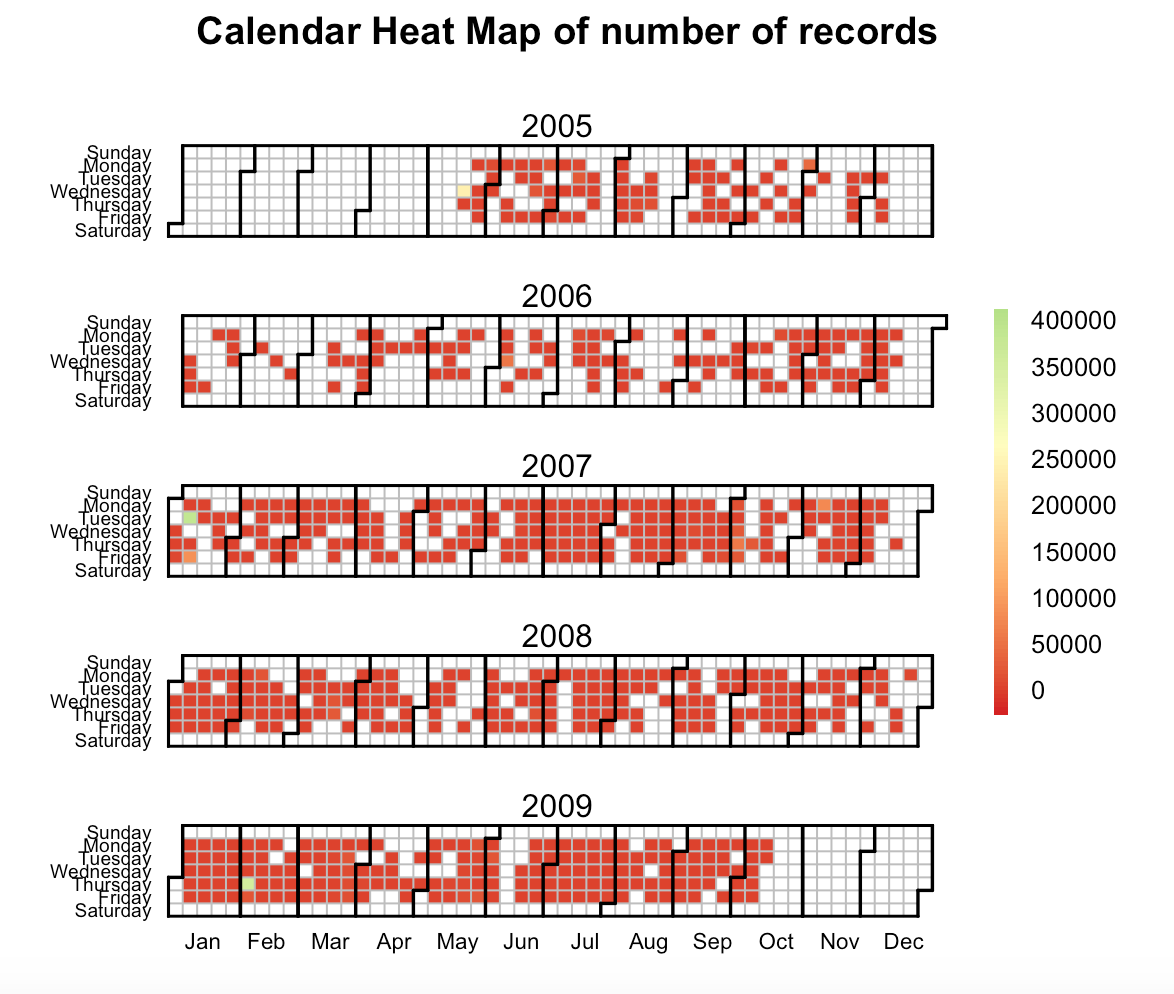
\includegraphics[width=0.5\textwidth]{pictures/biodiversity/heatmap.jpg} 
      \caption{Heat Calendar}
   \label{fig:heatcal}
\end{figure} 

 \subsection{Programming Hints}
 
 Some functions, such as mapgrid, are customizable.
 Arguments within the function, including \texttt{indf}, \texttt{ptype}, \texttt{title}, \texttt{bbox}, \texttt{legscale}, \texttt{collow}, \texttt{colhigh}, \texttt{mapdatabase}, \texttt{region}, and \texttt{customize}, allow the map to be configured to fit the data as desired.
 Using the function \texttt{help()} for mapgrid, and other functions, within the console of RStudio gives a more comprehensive overview of these functions. 
 
 Other functions can be used within the package bdvis.
 These functions include \texttt{tempolar}, \texttt{gettaxo}, and \texttt{taxotree}.
 Each function provides a different view of the data by compiling data that are not used in the other models, and by allowing users to view the same data through different means.
 

\section{Teaching Code}
This is the code shown in the above examples:

\begin{lstlisting}
#set working directory to data location
setwd("/Users/margauxwinter/Desktop/Rfolder/dwca-safring-v1.0")

#read data into RStudio
birds <- read.delim('occurrence.txt', quote='', stringsAsFactors=FALSE)

#configure data
conf <- list(Latitude='decimalLatitude',Longitude='decimalLongitude',
Date_collected='eventDate',Scientific_name='specificEpithet')
birds <- format_bdvis(birds, config=conf)
comp=bdcomplete(birds)

#visualize biodiversity data on the world map
mapgrid(comp,ptype='complete')

#create chronohorogram
chronohorogram(birds) 
comp=bdcomplete(birds,recs=5)

#create various distrigraphs
distrigraph(birds,ptype="cell",col="tomato") 
distrigraph(birds,ptype="species",ylab="Species") 
distrigraph(birds,ptype="efforts",col="red") 
distrigraph(birds,ptype="efforts",col="red",type="s") 

#create heat calendar
bdcalendarheat(birds) 
\end{lstlisting}

\section{Example Student Code}

The final deliverable should be submitted as visual models of the data in the form of distropraphs, maps, chronohorograms, and plots.
Use the arachnid data set downloaded from: \url{http://www.gbif.org/occurrence/download/0012867-160910150852091}

\begin{lstlisting}
#set working directory
setwd("/Users/margauxwinter/Desktop/Rfolder/
dwca-arc_national_survey_of_arachnida-v1.1")

#read in data set
spider <- read.delim('occurrence.txt', quote='', stringsAsFactors=FALSE)

#configure data to make it readable for bdvis package
conf <- list(Latitude='decimalLatitude',Longitude='decimalLongitude',
Date_collected='eventDate',Scientific_name='specificEpithet')
spider <- format_bdvis(spider, config=conf)
comp=bdcomplete(spider)

#begin functions for data visualization
mapgrid(comp,ptype='complete')
tempolar(spider, color="green", title="Arachnida daily", plottype="r", timescale="d") 
tempolar(spider, color="blue", title="Arachnida weekly", plottype="p", timescale="w") 
tempolar(spider, color="red", title="Arachnida monthly", plottype="r", timescale="m") 
chronohorogram(spider) 
comp=bdcomplete(spider,recs=5)
distrigraph(spider,ptype="cell",col="tomato") 
distrigraph(spider,ptype="species",ylab="Species") 
distrigraph(spider,ptype="efforts",col="red") 
distrigraph(spider,ptype="efforts",col="red",type="s") 
\end{lstlisting}
